\documentclass[
titlepage=firstiscover,
bibliography=totoc,
captions=tableheading,
]{scrartcl}

\usepackage[aux]{rerunfilecheck}



\usepackage{polyglossia}
\usepackage[autostyle]{csquotes}
\setmainlanguage{german}
\setotherlanguages{english, french}

\usepackage{microtype}

\usepackage{amsmath}
\usepackage{amssymb}
\usepackage{mathtools}

\usepackage{fontspec}

\usepackage[
  style=alphabetic,
]{biblatex}
\addbibresource{main.bib}

\usepackage[
math-style=ISO,
bold-style=ISO,
sans-style=italic,
nabla=upright,
partial=upright,
]{unicode-math}

\usepackage[
  locale=DE,
  separate-uncertainty=true,
  per-mode=symbol-or-fraction,
]{siunitx}

\sisetup{
locale=DE,
per-mode=symbol-or-fraction}

\usepackage[unicode]{hyperref}
\usepackage{bookmark}

\usepackage{graphicx}
\graphicspath{{build/}}

\usepackage{caption, booktabs}

\usepackage{grffile}
\usepackage{subcaption}
\usepackage{float}

\usepackage{xfrac}


\begin{document}

  \section{Aufgabe 2}

    \subsection{Aufgabe 2a}

    \begin{figure}[H]
      \centering
      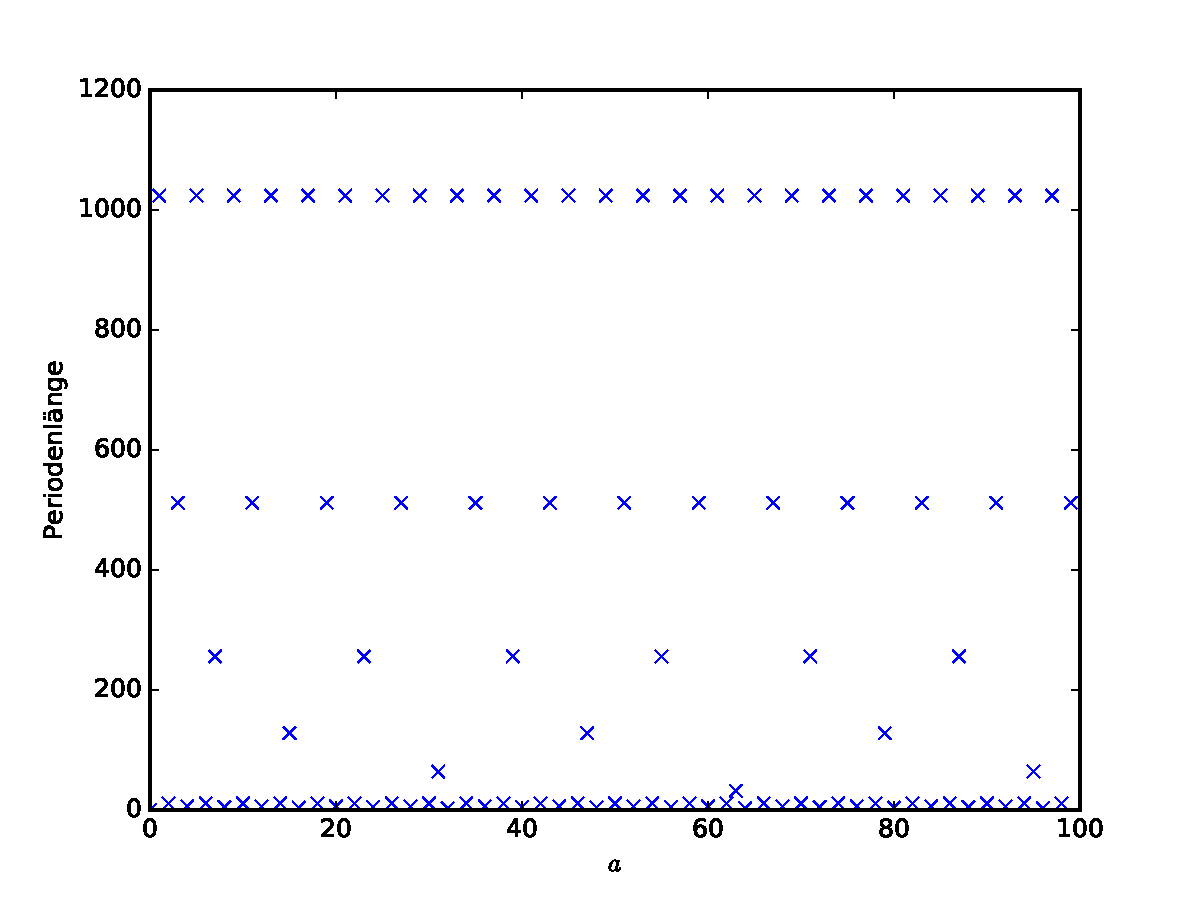
\includegraphics[height=10cm]{aPerioden.pdf}
      \caption{Periodenlänge des Zufallszahlgenerators in Abhängigkeit von $a$.}
      \label{fig:perioden}
    \end{figure}

    Die maximale Periodenlänge ist 1024(=$m.$) Die Periodenlänge ist für alle
    $4k+1\,(k\in\symbb{N}_0)$ maximal. Dies liegt daran, dass für diese Zahlen
    alle Kriterien für eine maximale Periodenlänge erfüllt sind:\\
    1) $b$ ist nicht 0.\\
    2) 1024 ist nicht durch 3 teilbar. Somit sind $b$ und $m$ teilerfremd.\\
    3) 2 ist der einzige Primfaktor von 1024. $4k+1-1$ ist immer eine gerade
    Zahl und somit durch 2 teilbar.\\
    4) 1024 ist durch 4 teilbar und $4k+1-1$ auch.\\

    \subsection{Aufgabe 2b}

    \begin{figure}[H]
      \centering
      \begin{subfigure}{0.48\textwidth}
        \centering
        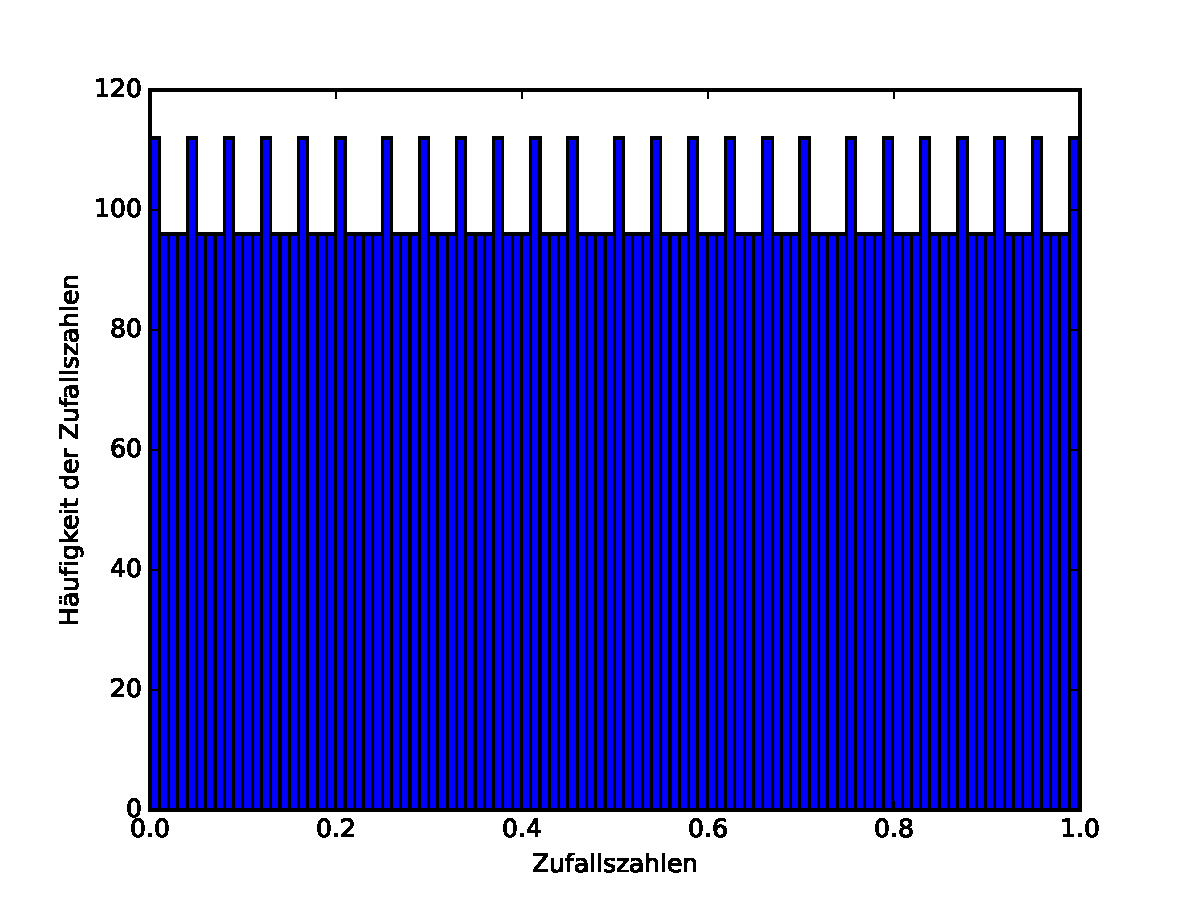
\includegraphics[height=5cm]{Histogrammb.pdf}
        \caption{Zufallszahlen für den Startwert 0.}
      \end{subfigure}
      \begin{subfigure}{0.48\textwidth}
        \centering
        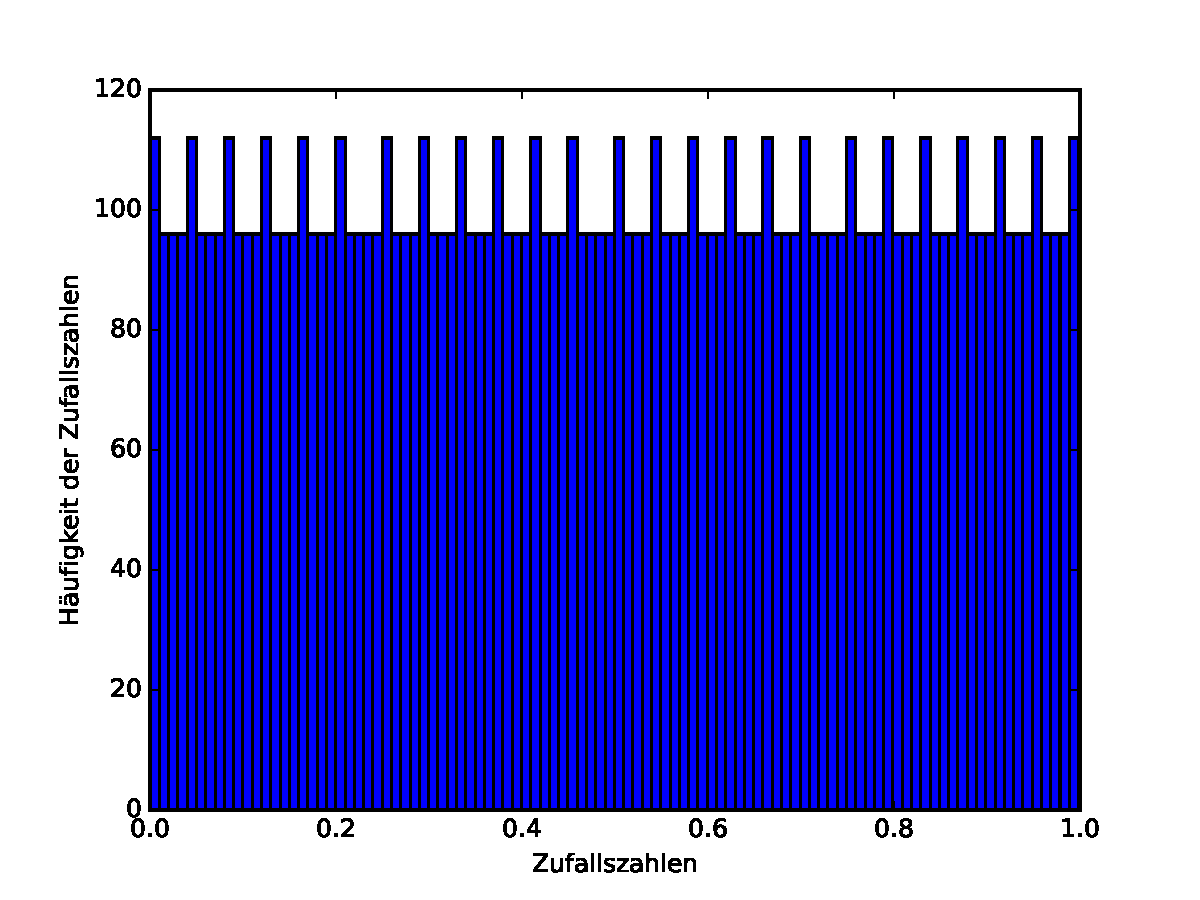
\includegraphics[height=5cm]{Histogrammb2.pdf}
        \caption{Zufallszahlen für den Startwert 1.}
      \end{subfigure}
      \begin{subfigure}{0.48\textwidth}
        \centering
        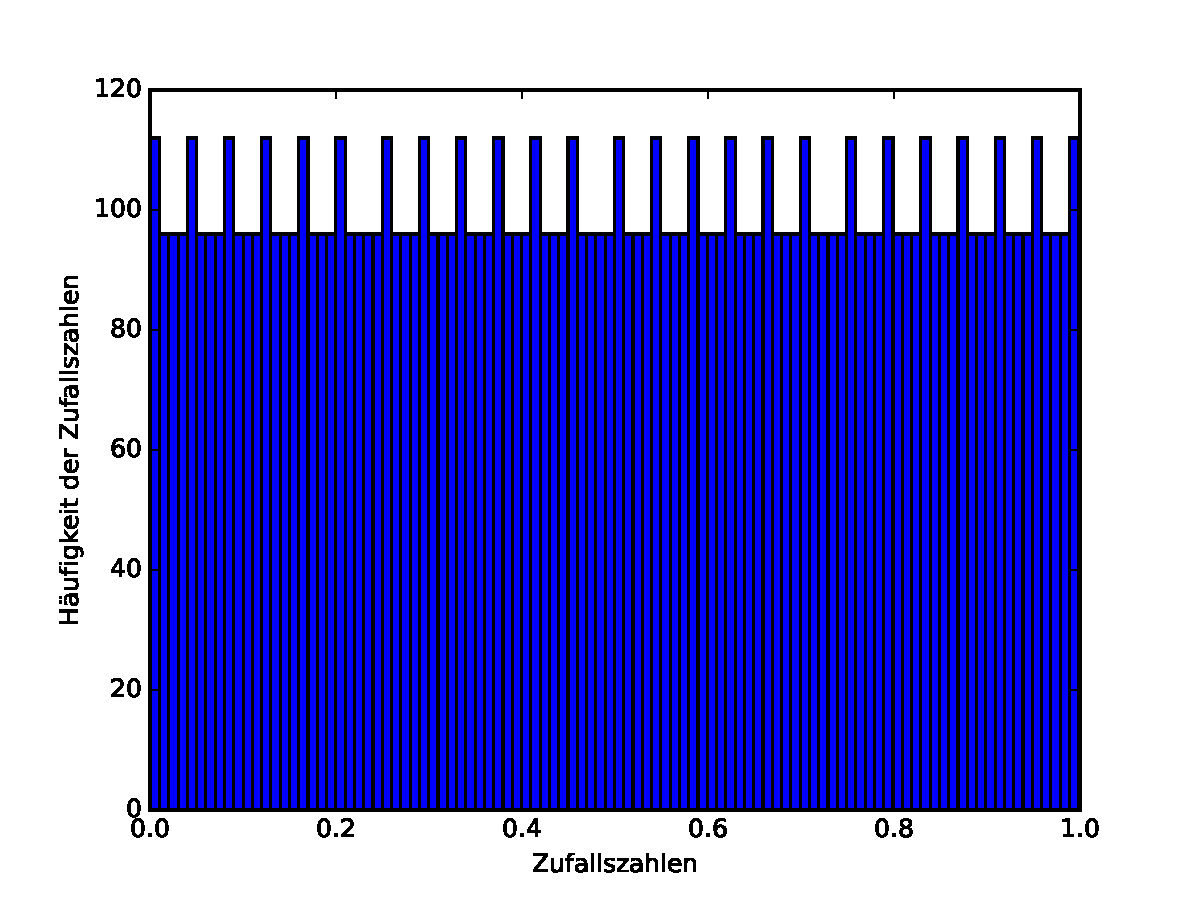
\includegraphics[height=5cm]{Histogrammb3.pdf}
        \caption{Zufallszahlen für den Startwert 2.}
      \end{subfigure}
      \begin{subfigure}{0.48\textwidth}
        \centering
        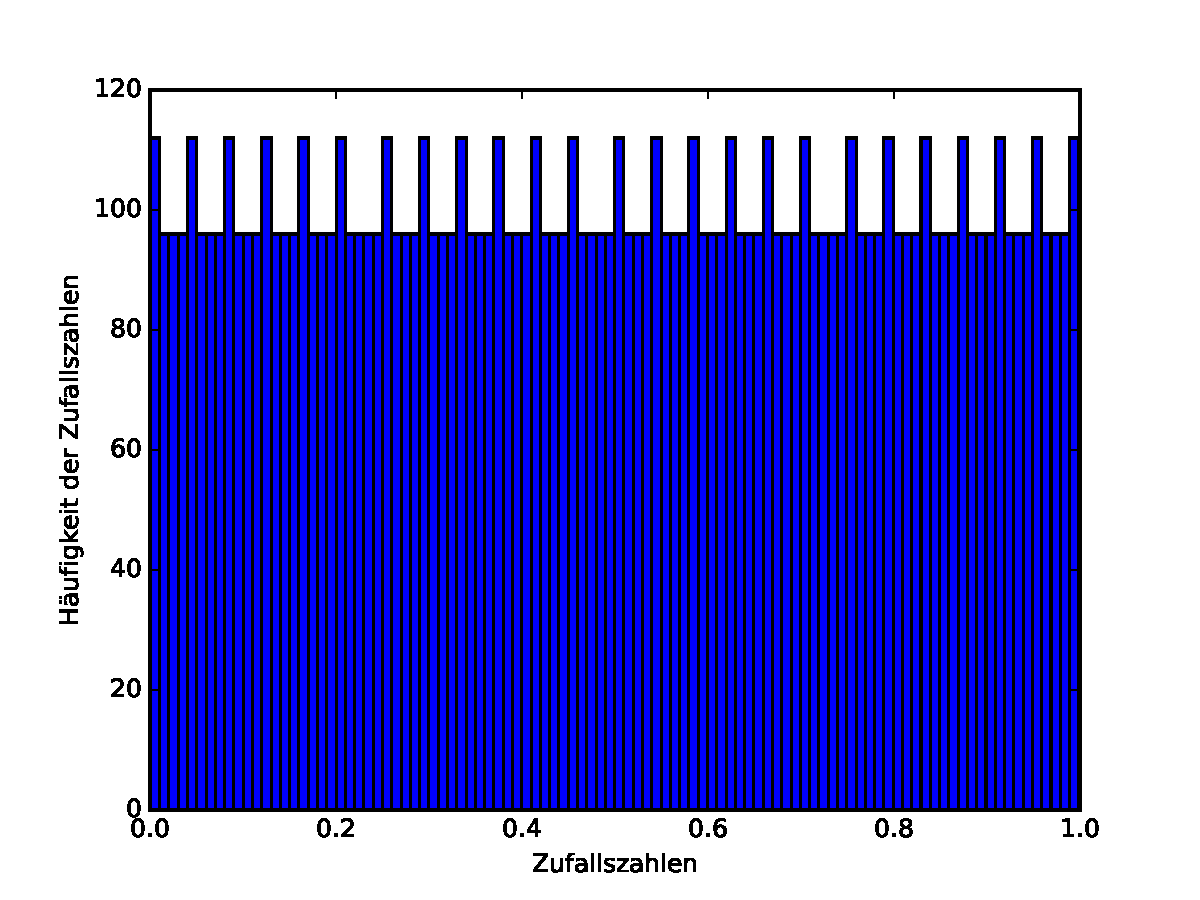
\includegraphics[height=5cm]{Histogrammb4.pdf}
        \caption{Zufallszahlen für den Startwert 100.}
      \end{subfigure}
      \begin{subfigure}{0.48\textwidth}
        \centering
        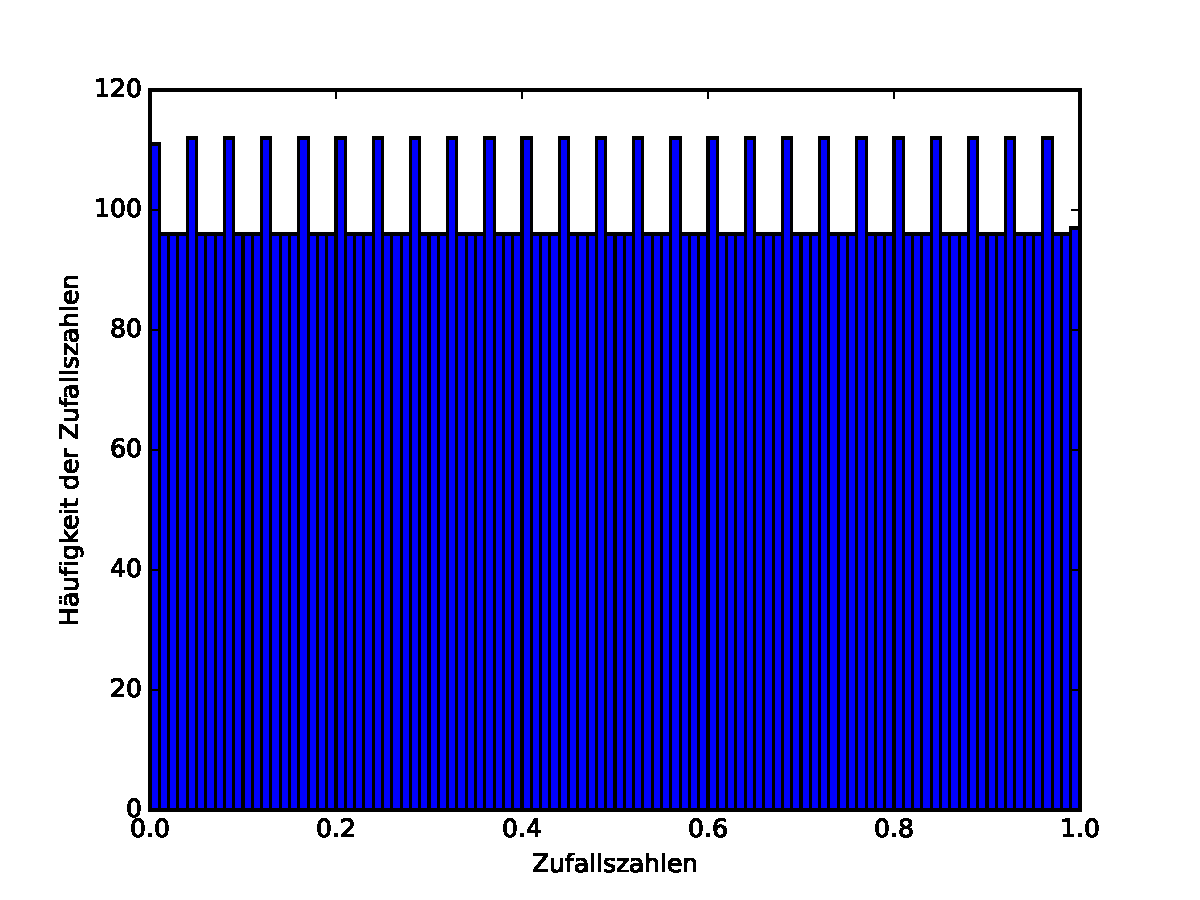
\includegraphics[height=5cm]{Histogrammb6.pdf}
        \caption{Zufallszahlen für den Startwert 10000.}
      \end{subfigure}
      \centering
      \begin{subfigure}{0.48\textwidth}
        \centering
        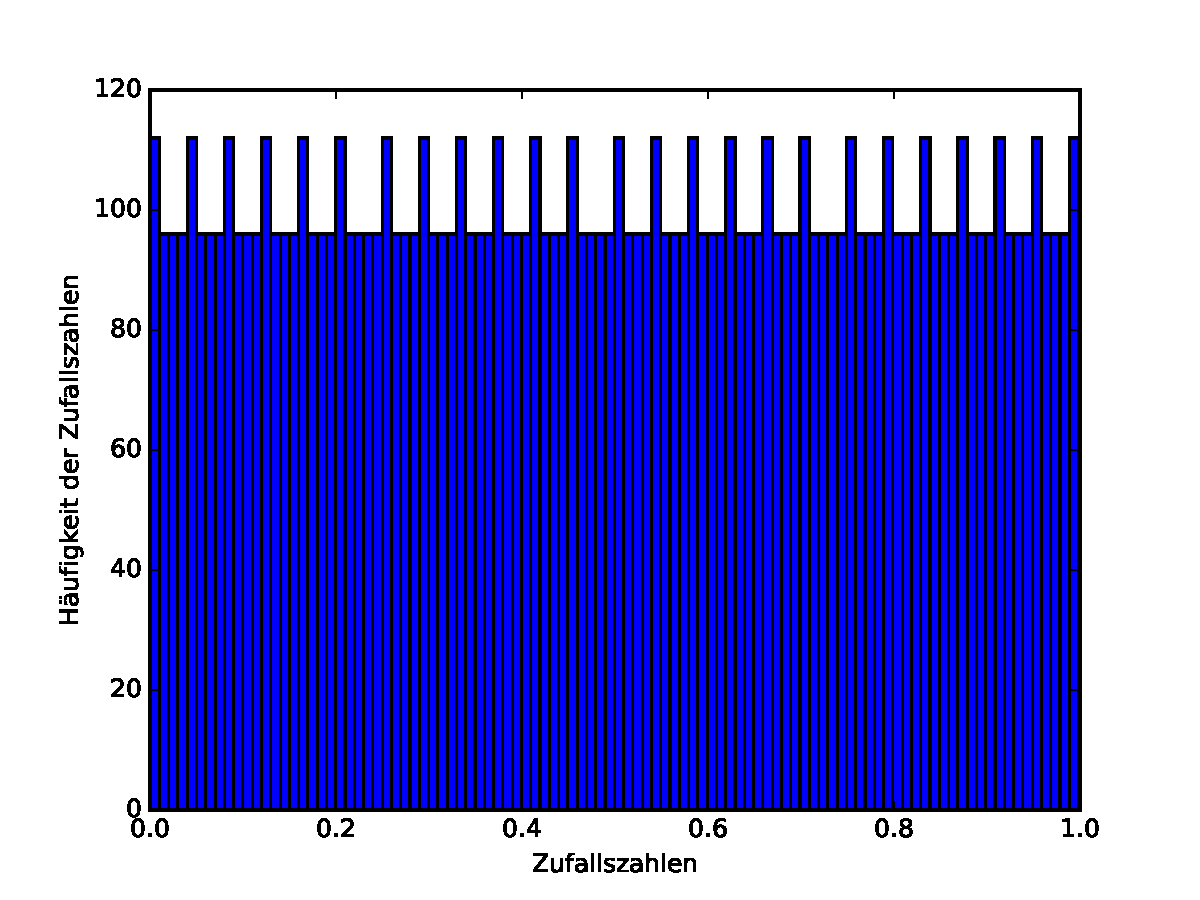
\includegraphics[height=5cm]{Histogrammb7.pdf}
        \caption{Zufallszahlen für den Startwert 0,5.}
      \end{subfigure}
      \begin{subfigure}{0.48\textwidth}
        \centering
        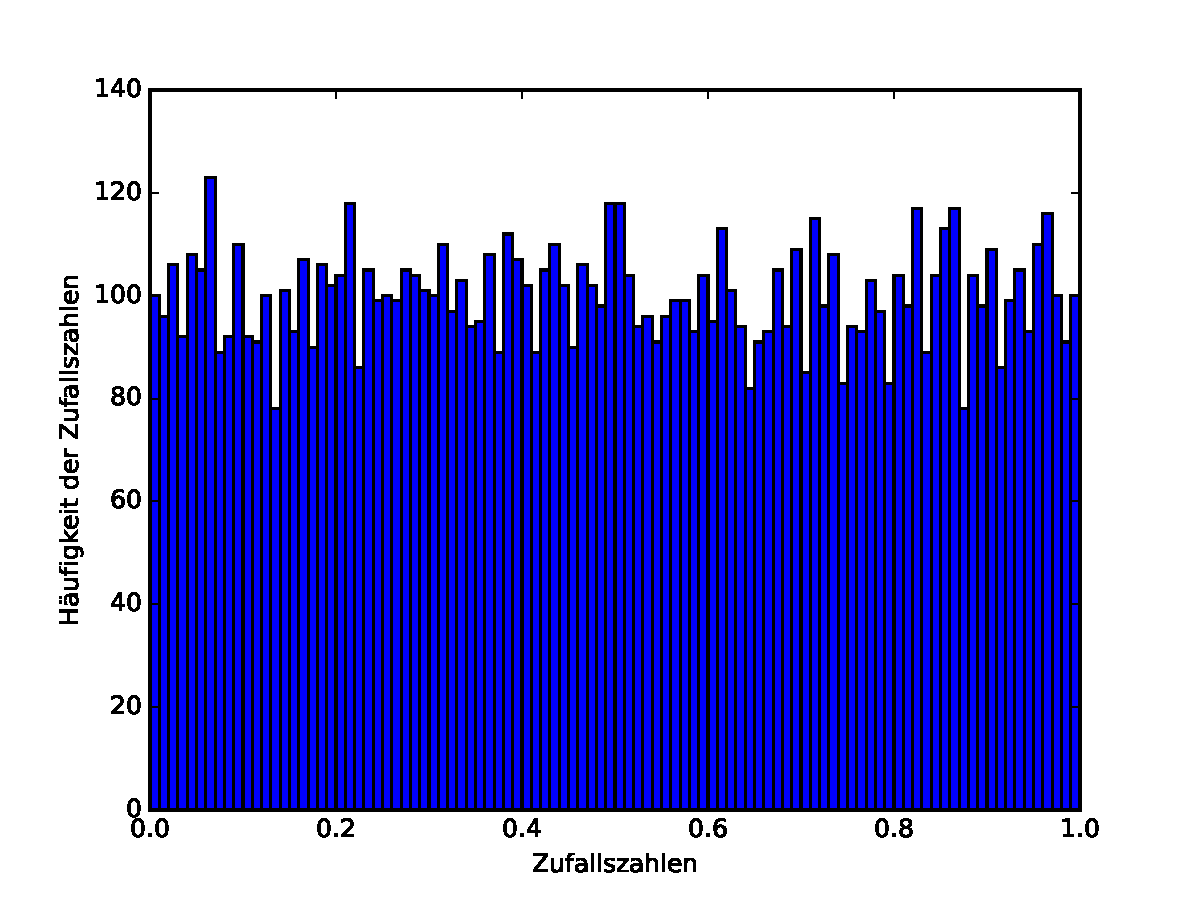
\includegraphics[height=5cm]{Histogrammb8.pdf}
        \caption{Zufallszahlen für den Startwert Pi.}
      \end{subfigure}
      \begin{subfigure}{0.48\textwidth}
        \centering
        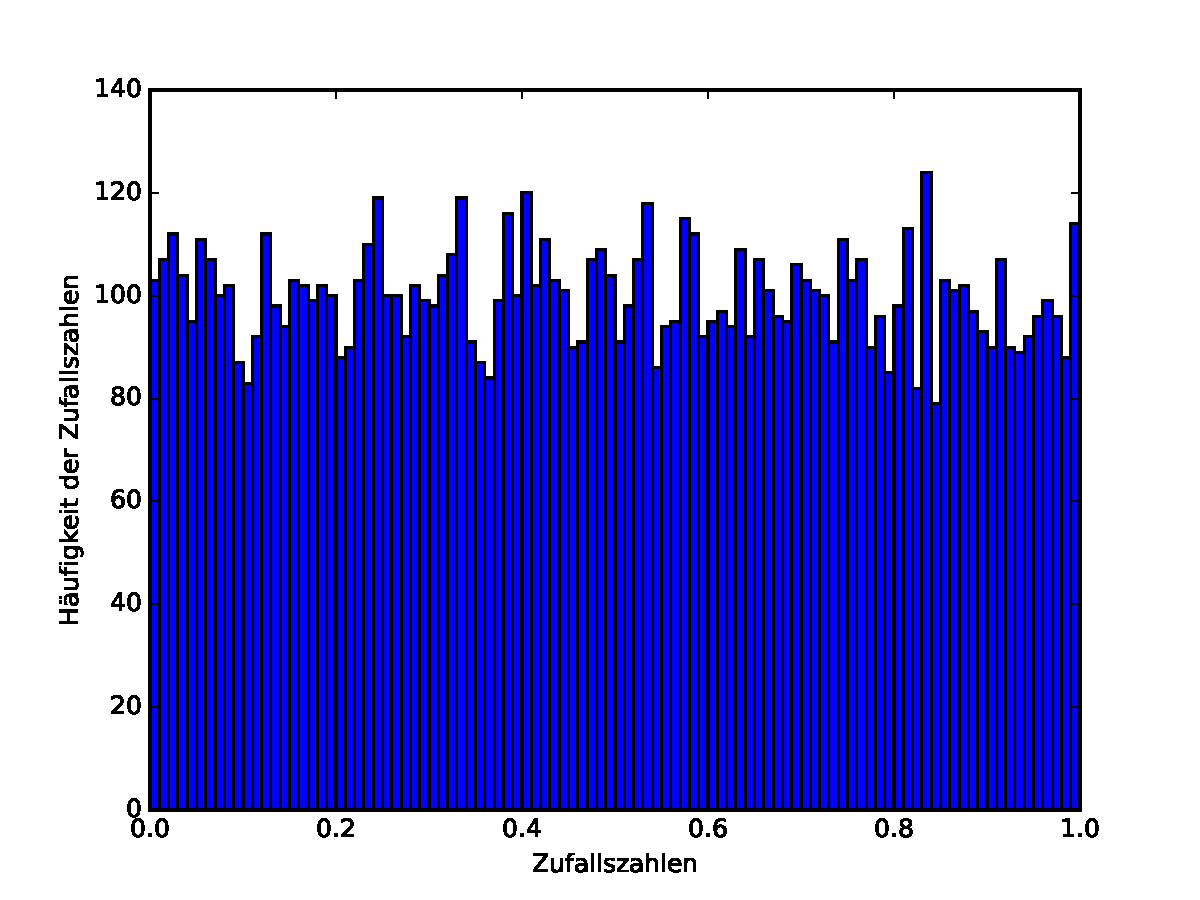
\includegraphics[height=5cm]{Histogrammb9.pdf}
        \caption{Zufallszahlen für den Startwert 3/7.}
      \end{subfigure}
      \caption{Histogramme von Zufallszahlen für unterschiedliche Startwerte.}
      \label{fig:histogramme}
    \end{figure}


    Es fällt auf, dass es bei ganzzahligen Werten keine Rolle für die Verteilung
    spielt, welcher Startwert ihr zugrunde liegt. Endliche Komma-Zahlen
    führen ebenfalls zur gleichen Verteilung. Nur bei Zahlen, die periodisch
    oder irrational sind, entsteht ein anderes Bild. Vielleicht ist dies
    aber auch auf Rundungen zurückzuführen. \\
    Es liegt kein guter Zufallsgenerator vor, da eine Periodizität zu erkennen
    ist.


    \subsection{Aufgabe 2c}

    \begin{figure}[H]
      \centering
      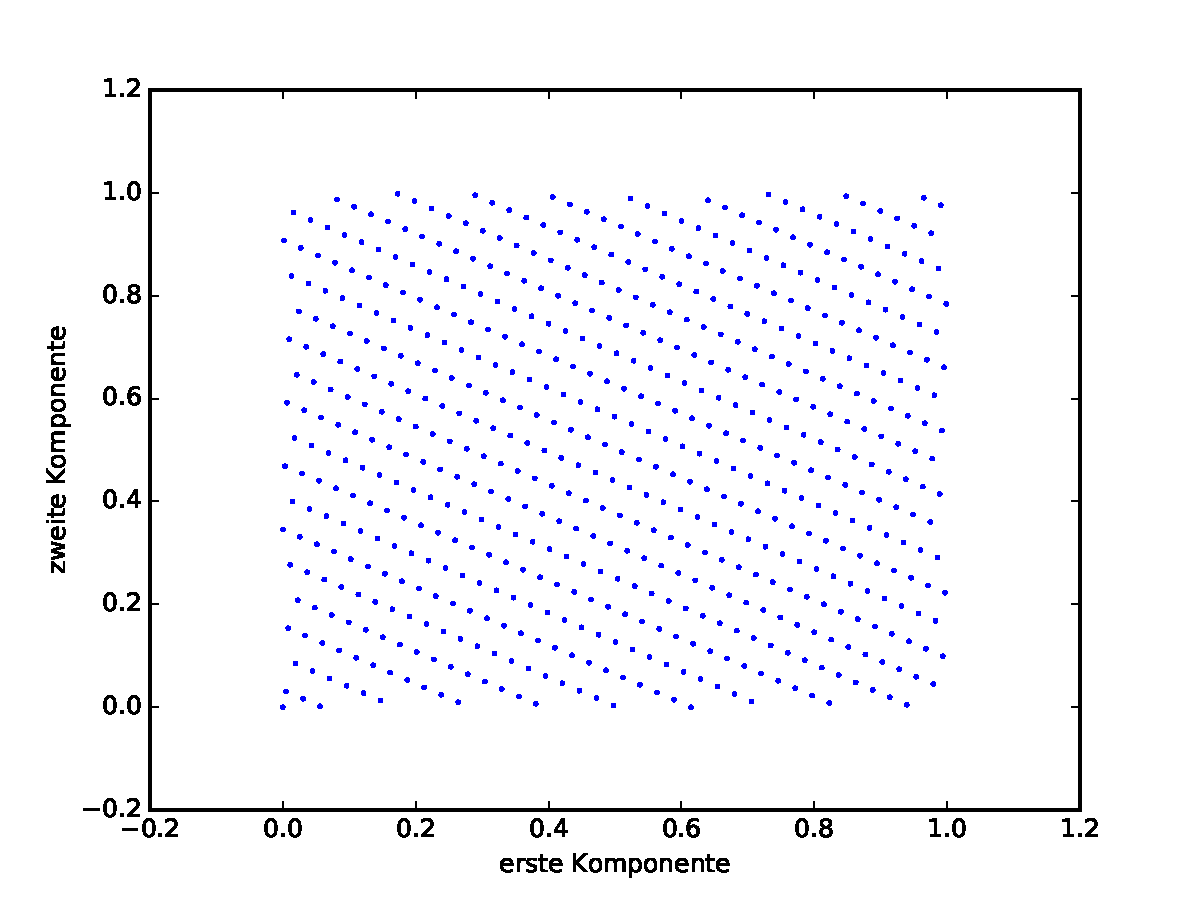
\includegraphics[height=7cm]{2D.pdf}
      \caption{Streudiagramm von Paaren aufeinanderfolgender Zufallszahlen
      (mit selbst programmiertem Generator erstellt).}
      \label{fig:2dscatter}
    \end{figure}

    \begin{figure}[H]
      \centering
      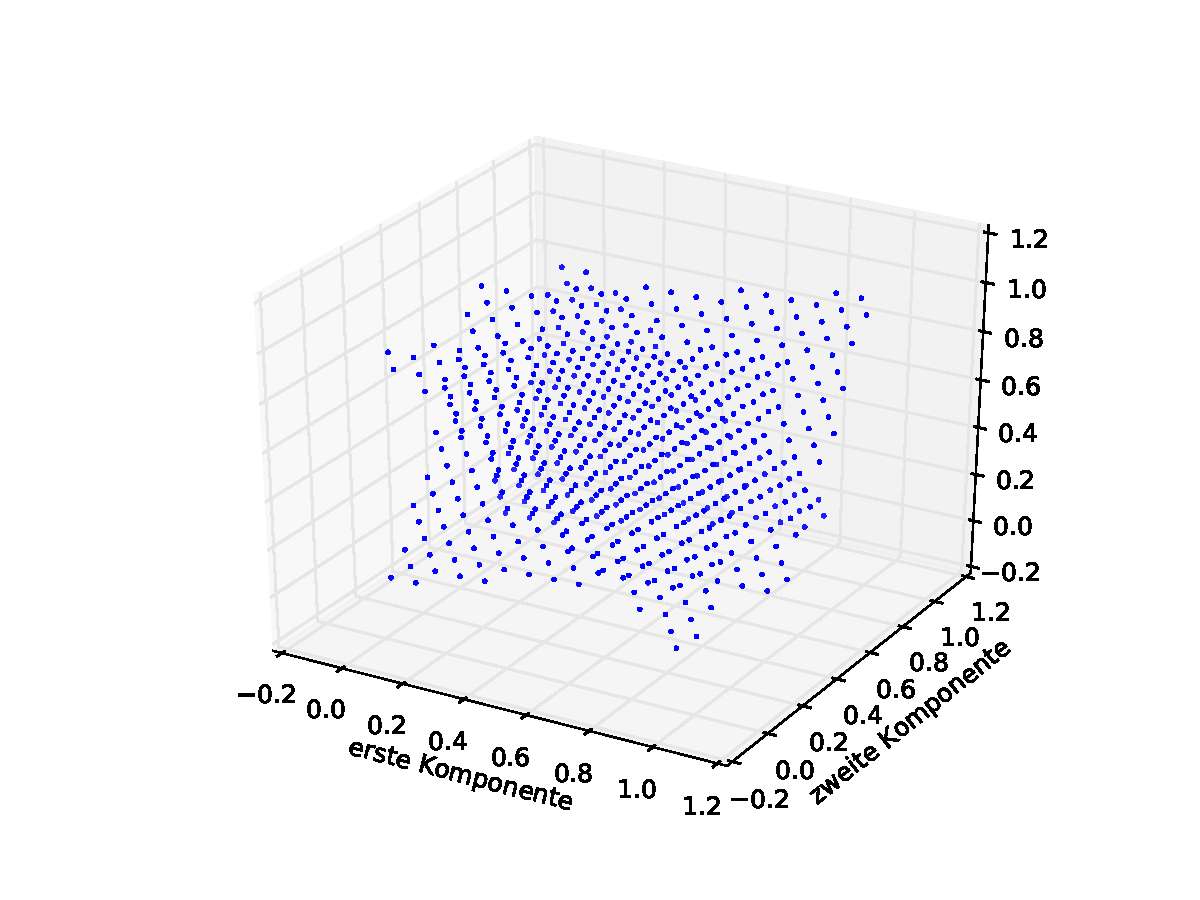
\includegraphics[height=7cm]{3D.pdf}
      \caption{Streudiagramm von Tripletts aufeinanderfolgender Zufallszahlen
      (mit selbst programmiertem Generator erstellt).}
      \label{fig:3dscatter}
    \end{figure}


    Auch hier ist leider eine gewisse Periodizität zu erkennen (Gitterform), weshalb
    sichtbar wird, dass der selbstprogrammierte Zufallsgenerator nicht den
    Anforderungen an einen guten Zufallsgenerator genügt.

    \subsection{Aufgabe 2d}

    \begin{figure}[H]
      \centering
      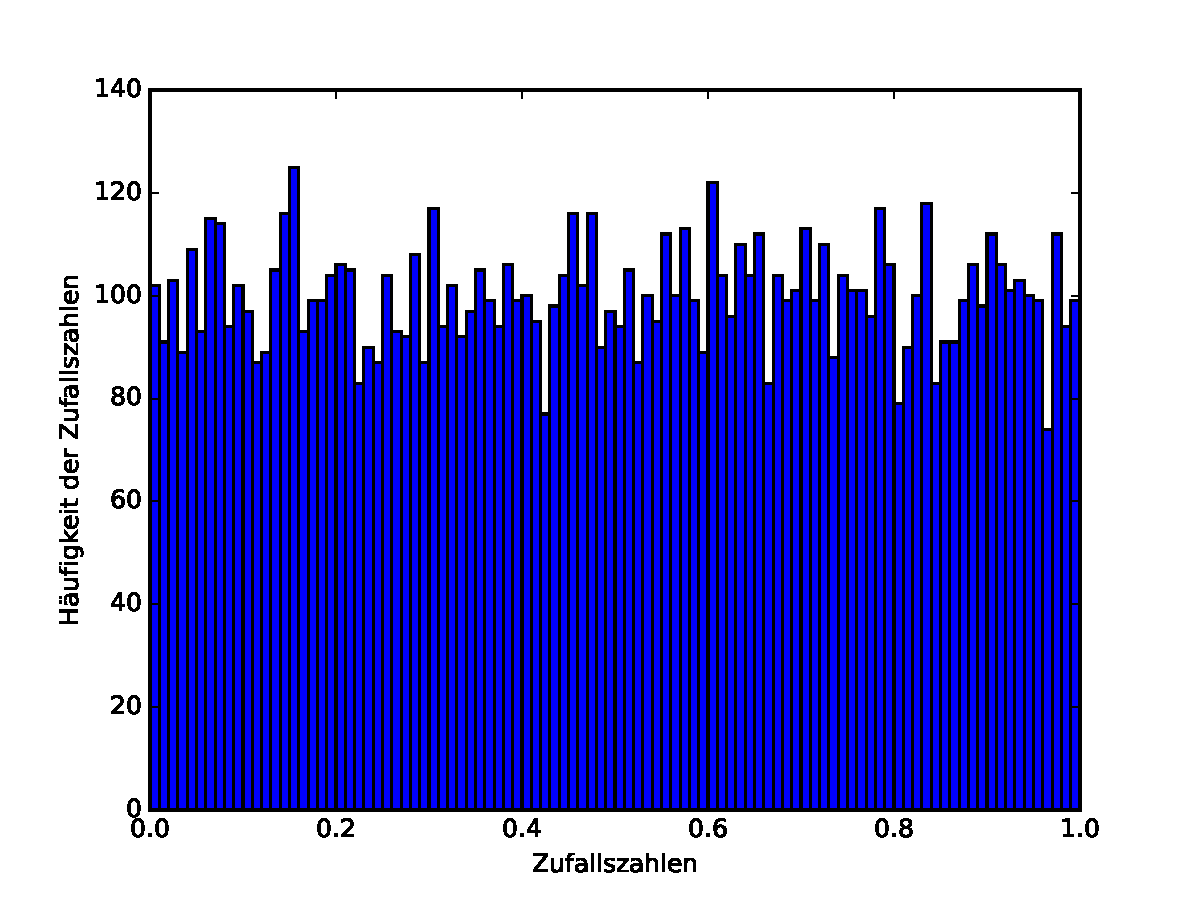
\includegraphics[height=7cm]{Histogrammd.pdf}
      \caption{Histogramm von Zufallszahlen
      (von numpy erstellt).}
      \label{fig:2dscatterd}
    \end{figure}

    Im Historgramm ist keine Periodizität mehr erkennbar.

    \begin{figure}[H]
      \centering
      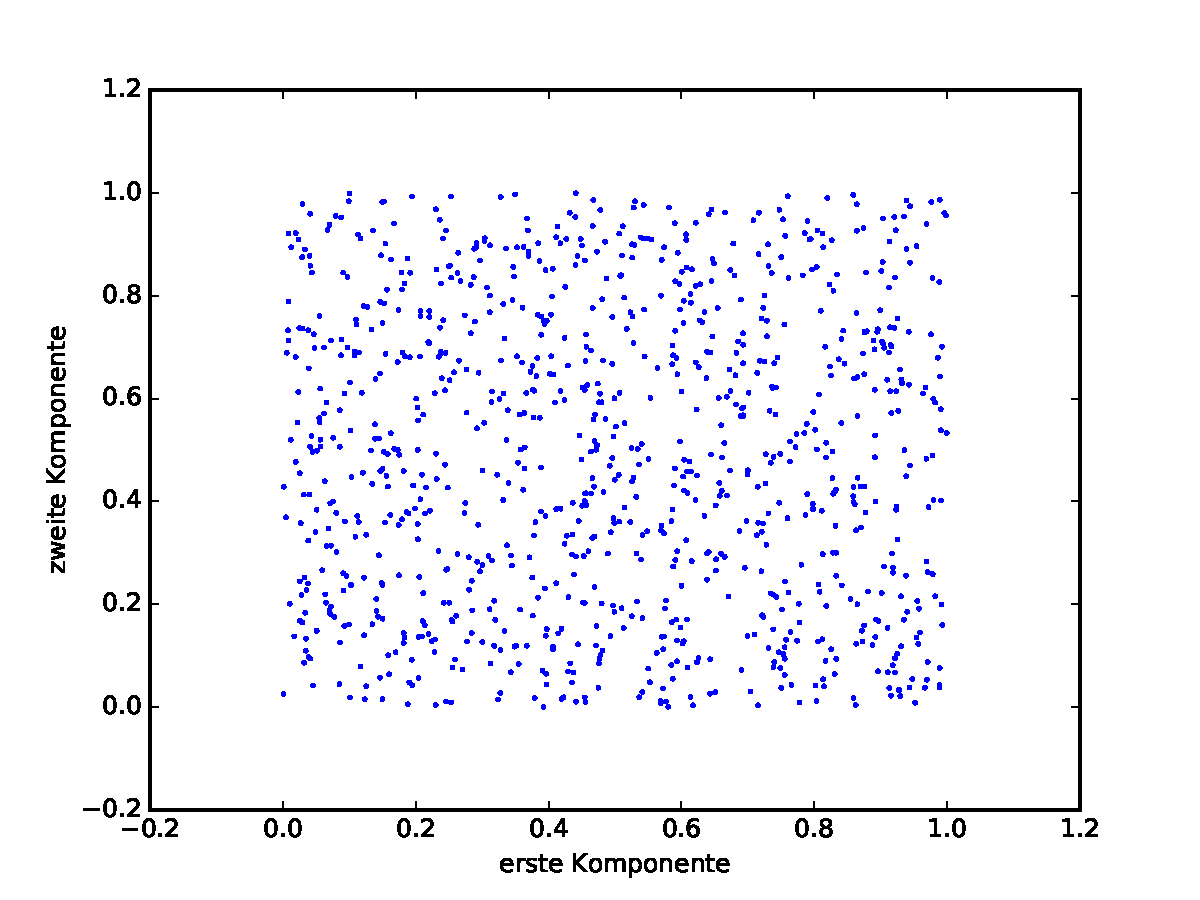
\includegraphics[height=7cm]{2Dd.pdf}
      \caption{Streudiagramm von Paaren aufeinanderfolgender Zufallszahlen
      (von numpy erstellt).}
      \label{fig:2dscatterd}
    \end{figure}

    \begin{figure}[H]
      \centering
      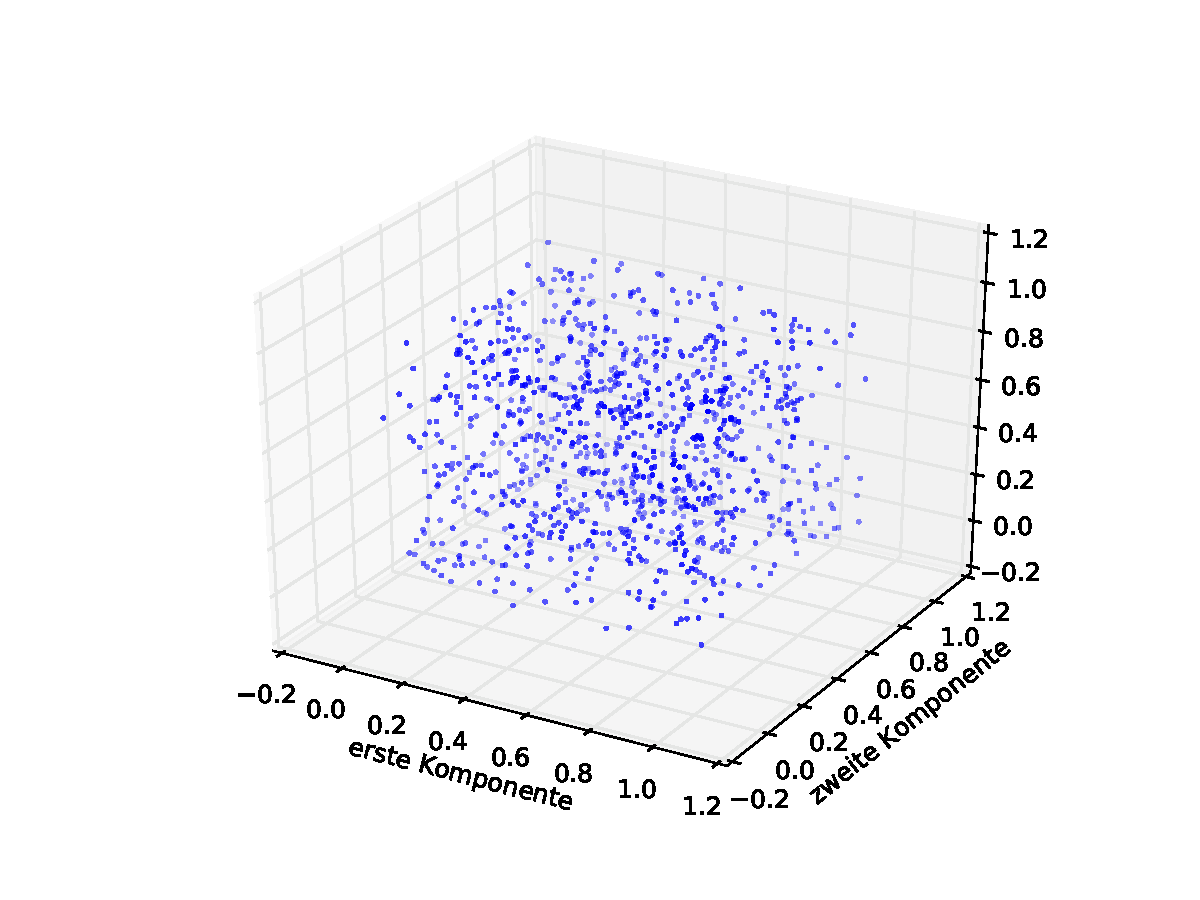
\includegraphics[height=7cm]{3Dd.pdf}
      \caption{Streudiagramm von Tripletts aufeinanderfolgender Zufallszahlen
      (von numpy erstellt).}
      \label{fig:3dscatterd}
    \end{figure}

    Die von numpy generierten Zufallszahlen sind nicht mehr auf klar erkennbaren
    Gitterzweigen, wie die des selbstprogrammierten Generators.

    \subsection{Aufgabe 2e}

    Parameter:\\
    $a=3$\\
    $b=3$\\
    $m=1024$\\

    Wie oft unter den 1024 Zahlen die Zahl $\frac12$ zu finden ist,
    hängt vom Startwert ab.  \\
    Bei einigen Startwerten (wie zum Beispiel 2) ist der Generator
    gar nicht in der Lage, die Zahl überhaupt zu erstellen.\\
    Für den Startwert 348672 kommt $\frac12$ jedoch einmal vor,
    und für den Startwert 511 ist die Zufallszahl gleich zweimal inerhalb
    der Werte zu finden.






























\end{document}
